\providecommand{\pdfxopts}{a-1b,cyrxmp}
\providecommand{\thisyear}{2022}
\immediate\write18{rm \jobname.xmpdata}%  uncomment for Unix-based systems
\begin{filecontents*}{\jobname.xmpdata}
	\Title{Проект рабочей программы дисциплины "Цифровая электроника" \textemdash\thisyear}
\Author{Артем Николаевич Прокшин}
\Creator{pdfTeX + pdfx.sty with options \pdfxopts }
\Subject{Проект рабочей программы дисциплины "Цифровая электроника"}
\Keywords{цифровая и микропроцессорная техника, ковариантные и контравариантные координаты, MexBIOS Development Studio, электрические машины}
\CoverDisplayDate{март \thisyear}
\CoverDate{2022-05-16}
\Copyrighted{True}
\Copyright{Public Domain}
\CopyrightURL{http://github.com/trot-t}
\Creator{pdfTeX + pdfx.sty with options \pdfxopts }
\end{filecontents*}

\documentclass[14pt, aspectratio=169]{beamer}

\pdfcompresslevel=9

\usepackage[\pdfxopts]{pdfx}[2016/03/09]
\PassOptionsToPackage{obeyspaces}{url}
\let\tldocrussian=1  % for live4ht.cfg

\usepackage[T2A]{fontenc}
\usepackage[utf8]{inputenc}
\usepackage[english,russian]{babel}
\usepackage{booktabs}
\usepackage{tikz}
\usepackage[european,cuteinductors,smartlabels]{circuitikz}
\usetikzlibrary{arrows.meta, shadows}

\usepackage{amssymb,amsfonts,amsmath,mathtext}
\usepackage{amssymb}
\usepackage{cite,enumerate,float,indentfirst}
\usepackage{cancel}
\usepackage{csquotes}
\newcommand{\quotes}[1]{``#1''}
\usetikzlibrary{calc}

\usepackage{advdate}

%\usepackage{pgfplots}
%\usepackage[left=1cm,right=1cm, top=1cm,bottom=1cm,bindingoffset=0cm]{geometry}

% Beamer — верстаем презентации  https://habrahabr.ru/post/145523/ 
\graphicspath{{images/}}

\usetheme{Pittsburgh}
\usecolortheme{whale}
%\usetheme{SaintPetersburg}  % находится в пакете texlive-beamertheme-saintpetersburg

%\usetheme{Darmstadt}
%\usefonttheme[onlylarge]{structurebold}
%\setbeamerfont*{frametitle}{size=\normalsize,series=\bfseries}
%\setbeamertemplate{navigation symbols}{}



\setbeamercolor{footline}{fg=blue}
\setbeamertemplate{footline}{
\leavevmode%
\hbox{%
\begin{beamercolorbox}[wd=.333333\paperwidth,ht=2.25ex,dp=1ex,center]{}%
Прокшин А.Н. и др.
\end{beamercolorbox}%
\begin{beamercolorbox}[wd=.333333\paperwidth,ht=2.25ex,dp=1ex,center]{}%
Санкт-Петербург, 2022
\end{beamercolorbox}%
\begin{beamercolorbox}[wd=.333333\paperwidth,ht=2.25ex,dp=1ex,right]{}%
Стр. \insertframenumber{} из \inserttotalframenumber \hspace*{2ex}
\end{beamercolorbox}}%
\vskip0pt%
}

\definecolor{innopolisGreen}{RGB}{21,176,18}

\setbeamercolor{title}{bg=innopolisGreen,fg=black!15}


\setbeamercolor{alerted text}{fg=red!70!yellow!70,bg=black}

\definecolor{spbuWhite1}{RGB}{245,246,245}
\beamertemplatesolidbackgroundcolor{spbuWhite1}
\setbeamercolor{frametitle}{bg=spbuWhite1,fg=innopolisGreen}


\usefonttheme[onlymath]{serif} % в формулах использовать текст с засечками

\begin{document}
\title{\small{
Проект рабочей программы дисциплины \enquote{Цифровая электроника}
для подготовки бакалавров по направлению
            13.03.02 \enquote{Электроэнергетика и электротехника}
по профилю
\enquote{Электропривод и автоматика}
}}
\author{\small{%
\emph{авторы:}
\emph{}~ст.преп. Прокшин Артем Николаевич}}


%\titlegraphic{%
%\includegraphics[width=.7\linewidth]{logo}}

%\othergraphic{%
%\includegraphics[width=.7\linewidth]{logo}}

%\leftcolumnwidth{.2\linewidth}
%$\middlecolumnwidth{.6\linewidth}
%$\rightcolumnwidth{.2\linewidth}


\institute{Санкт-Петербургский государственный электротехнический университет «ЛЭТИ» им. В.И. Ульянова (Ленина)}
\vspace{30pt}%

\vspace{60pt}%

\AdvanceDate[-1] % печатаю в субботу а нужна пятница
%\date{\small{Санкт-Петербург, 2022}}

\AtBeginSection{
	\begin{frame}
		\frametitle{Содержание}
		\tableofcontents[currentsection]
	\end{frame}
}

\begin{frame}
\titlepage	
\end{frame}

%\begin{frame}
%        \frametitle{Содержание}
%        \tableofcontents[currentsection] 
%\end{frame}
\begin{frame}
%\frametitle{\small Цели, к которым стремились при реализации курса} 
\frametitle{\begin{tabular}{lp{100pt}r}Актуальность&&
\includegraphics[width=0.25\linewidth]{logo2}\end{tabular}} 
\begin{itemize}
	\item упрощение системы управления с использованием ковариантных (измеряемых) и контравариантных (неизмеряемых) координат;
%\item использование дипломных проектов студентов; % предыдущих выпусков;
\item создание мобильных лабораторных стендов; % по тематике кафедры с перспективой на использование российских разработок;
\item использование российского программного обеспечения;
\item использование российских микроконтроллеров в части задач 
%\item оформление УМКД;
%\item ... будет сформулирована в результатах.
\end{itemize}
\end{frame}

%\begin{frame}
%\frametitle{Аннотация дисциплины}
%Изучаются архитектура современных цифровых систем управления с микроконтроллерами, основные этапы анализа, синтеза и проектирования таких систем.
%Подробно рассматриваются вопросы математического описания систем управления с микроконтроллерами, анализ и синтез с использованием методов как классической, так и современной теории управления. 
%Теоретическая часть курса сопровождается практическими и лабораторными занятиями для практического освоения изученного материала.
%\end{frame}

%\begin{frame}
%\frametitle{Компетенции}
%\begin{itemize}
%\item{ОПК-1} Способен осуществлять поиск, обработку и анализ информации из различных источников и представлять ее в требуемом формате с использованием информационных, компьютерных и сетевых технологий 
%\item{ОПК-2} Способен применять соответствующий физико-математический аппарат, методы анализа и моделирования, теоретического и экспериментального исследования при решении профессиональных задач
%\end{itemize}
%\end{frame}

\begin{frame}
\frametitle{\begin{tabular}{lp{100pt}r}Компетенции&&
\includegraphics[width=0.25\linewidth]{logo2}\end{tabular}}
\vspace{-0.3cm}
{\footnotesize Компетенция {\bf ОПК-2} Способен применять соответствующий физико-математический аппарат, методы анализа и моделирования, теоретического и экспериментального исследования при решении профессиональных задач}
\vspace{-0.7cm}
\begin{columns}[t]
\hspace{-1.2cm}
    \column{.3\textwidth}
    \footnotesize
    \begin{exampleblock}{\footnotesize Знать}
       \begin{itemize}
          \item геометрические основы измерения трехфазного тока
          \item\colorbox{yellow}{\parbox[t]{1\textwidth}{среды разработки и моделирования встроенного программного обеспечения систем управления электродвигателями, технологическими комплексами}}
       \end{itemize}
    \end{exampleblock}
   \column{.3\textwidth}
    \footnotesize
    \begin{exampleblock}{\footnotesize Уметь}
      \begin{itemize}
        \item \colorbox{yellow}{\parbox[t]{\textwidth}{применить среды разработки и моделирования MexBios Development Studio, SimInTech, Texas Instrument CCS, Motor Control Workbench, GCC toolchain для 
 создания программы управления инвертором электрическими машинами}}
     \end{itemize}
    \end{exampleblock}
   \column{.28\textwidth}
    \footnotesize
    \begin{exampleblock}{\footnotesize Владеть }
      \begin{itemize}
        \item \colorbox{yellow}{\parbox[t]{\textwidth}{настройкой взаимодействия сред разработки с микроконтроллером и конечным оборудованием, отладка, поиск и устранение неисправностей в программе}}
%электродвигателем, идентифицировать и устранить неисправность, скорректировать фактический режим электродвигателя}
     \end{itemize}
    \end{exampleblock}
\end{columns}
\end{frame}


\begin{frame}
\frametitle{\begin{tabular}{lp{10pt}r}\parbox{0.65\textwidth}{\small Используемые в обучении информационные и \enquote{сквозные} технологии, цифровые инструменты}&&
\includegraphics[width=0.25\linewidth]{logo2}\end{tabular}}
\footnotesize
\begin{itemize}
\item\colorbox{yellow}{Современные проблемы инфраструктуры электродвижения} \href{https://www.np-sr.ru/}{\quotes{НП Совет рынка}}, \href{https://www.atsenergo.ru}{АО \quotes{АТС}}, криптография ГОСТ, PKI, ocsp, проверка электронных подписей
\item\colorbox{yellow}{11 тем связанных с изображающими векторами} Современная геометрия, ковариантные и контравариантные координаты векторов, двойственные дуальные базисы, \url{overleaf.com}, \url{geogebra.com}, \url{www.latex4technics.com}, \href{https://www.tflex.com}{T-Flex}.
\item\colorbox{yellow}{Преобразование базисов и координат из одной системы в другую} Матричный анализ, \href{http://www.reduce-algebra.com/}{reduce-algebra}, \href{https://maxima.sourceforge.io/ru/}{maxima}, \url{overleaf.com}, \url{geogebra.com}, \url{www.latex4technics.com}, \href{https://www.tflex.com}{T-Flex}.
\item\colorbox{yellow}{Интегрированные системы программирования микроконтроллеров} \href{https://mechatronica-pro.com/ru}{MexBIOS}, \href{http://motorcontrol.ru}{среда НПФ Вектор}, \href{ti.com}{CodeComposerStudio}, \href{st.com}{STM32CubeIDE}, arm-none-eabi-* toolchain, st-link, DFU
%\url{www.latex4technics.com?note=409W}


\end{itemize}
\end{frame}


\begin{frame}
\frametitle{\begin{tabular}{lp{10pt}r}\parbox{0.65\textwidth}{\small Используемые в обучении информационные и \enquote{сквозные} технологии, цифровые инструменты}&&
\includegraphics[width=0.25\linewidth]{logo2}\end{tabular}}
\footnotesize
\begin{itemize}
\item\colorbox{yellow}{Принципы работы одно- и трех-фазного мостового инвертора напряжения} Моделирование работы инвертора  
\href{http://www.raps-lab.eltech.ru/cgi-bin/circuit.pl}{на сервисе кафедры РАПС},
\href{http://www.geda-project.org/}{geda}, \href{http://ngspice.sourceforge.net/}{ngspice}, \href{easygeda.com}{easyEDA}, \href{https://simintech.ru/}{SimInTech}
\item\colorbox{yellow}{Отладка программ и блоков в МехBIOS, SimInTech и в облачных сервисах} \href{https://www.mycompiler.io/new/c}{песочница C},
\href{http://cpp.sh/}{песочница С++}, gcc, \url{overleaf.com} 
\item\colorbox{yellow}{Отчеты оформляются исключительно по ЕСКД}  latex, \url{overleaf.com} 
\item\colorbox{yellow}{Исходные коды блоков, шаблоны заданий и отчетов располагаются в системе} \colorbox{yellow}{контроля версий git с настроенной связью в overleaf и C-песочницами} \href{https://git-scm.com}{Git}, \href{https://github.com/trot-t}{github.com}, \href{https://www.mycompiler.io/new/c}{песочница C}, \url{overleaf.com}

%\item{\color{red}Измеряемые мгновенные значения токов и напряжений и их связь с ковариантными координатами} \url{https://www.mycompiler.io/new/c}
%\url{http://cpp.sh/} \url{overleaf.com}


\end{itemize}
\end{frame}


\begin{frame}
\frametitle{\begin{tabular}{lp{10pt}r}\parbox{0.65\textwidth}{\small Используемые в обучении информационные и \enquote{сквозные} технологии, цифровые инструменты}&&
\includegraphics[width=0.25\linewidth]{logo2}\end{tabular}}
\vspace{-0.5cm}
\begin{columns}[t]
    \column{.50\textwidth}
    \footnotesize
    \begin{exampleblock}{\footnotesize Современные проблемы инфраструктуры электродвижения} %преобразователей электрической энергии}
       \begin{itemize}
          \item недостаточная мощность и кол-во зарядных станций (преобразователей электрической энергии) для электрических автомобилей, судов 
          \item логистика и планирование заряда/разряда батарей автономного электрического транспорта
          \item \colorbox{yellow}{\parbox{0.8\textwidth}{транспондеры, смартконтракты, российская криптография, блокчейн}}
       \end{itemize}
    \end{exampleblock}
   \column{.50\textwidth}
    \footnotesize
    \begin{exampleblock}{\footnotesize Передача активной и реактивной мощности между электрической машиной и промышленной сетью}
      \begin{itemize}
        \item изображающие векторы напряжения и тока
        \item реактивная мощность стекает с повышенного напряжения
        \item вектор напряжения передающей активную мощность электрической машины обгоняет вектор приемника
        \item вектор тока одинаков для обеих машин 
      \end{itemize}
    \end{exampleblock}
\end{columns}
\end{frame}


\foreach \ThemeA\ItemsA\ThemeB\ItemsB in {
Принципы работы однофазного мостового инвертора напряжения 
/{
   чисто активная нагрузка,
   нагрузка или источник содержит индуктивность или дроссель,
   работа обратного диода,
   передаваемая мощность при медленно меняющемся токе и быстро меняющемся напряжении в зависимости от скважности
}/
Принципы работы трехфазного мостового инвертора напряжения
/{
   порядок переключения ключей,
   график токов в фазах при активной нагрузке,
   графики фазных и линейных напряжений,
   изображающие вектора фазных и линейных напряжений и токов
},
Работа ключей при векторной широтно-импульсной модуляции в трехфазном мостовом инверторе напряжения
/{
   таблица векторов состояний,
   нулевой вектор состоит из 2-х состояний,
   изображающий вектор как центр тяжести состояний взвешенных по времени нахождения в данном состоянии,
   потенциалы фаз и нуля
}/
Синусоидальная широтно-импульсная модуляция в однофазном или трехфазном мостовом инверторе напряжения
/{
   наличие реального или \enquote{виртуального} нулевого провода,
   отличие активной мощности при синусоидальной и векторной широтно-импульсной модуляциях
},
Системы координат. Преобразование базисов и координат из одной системы в другую
/{
   разложение вектора по координатным осям по правилу параллелограмма,
   матрица преобразования
}/
{Системы координат в современной геометрии, косоугольная система координат, ковариантные и контравариантные координаты в косоугольной системе координат}
/{
   \colorbox{yellow}{\parbox{0.7\textwidth}{формула длины вектора в косоугольной системе координат $|\vec{x}|=\sqrt{x_1x^1 + x_2x^2}$}},
   \colorbox{yellow}{\parbox{0.82\textwidth}{скалярное произведение двух векторов $\vec{x}\cdot\vec{y} = x_iy^i =  x^iy_i$}},
   \colorbox{yellow}{правило Эйнштейна},
   сравнение с прямоугольной декартовой системой координат
%   \it метрический тензор
},
Измеряемые мгновенные значения токов и напряжений и их связь с ковариантными координатами
/{
   преобразование Блонделя $\vec{i} = \frac{2}{3}\left(i_a \vec{e}_a + i_b \vec{e}_b + i_c \vec{e}_c\right)$,
   \colorbox{yellow}{\parbox{0.82\textwidth}{формула для $\vec{i}$ в симметричной системе координат, полусумма контравариантных координат равна контравариантной координате
         $$
             i_a = \frac{1}{2}\left(i^a_\text {в осях AB} + i^a_\text{ в осях AC} \right)
         $$}}
}/
управление ШИМ через центр тяжести весов векторов состояния инвертора и связь с контравариантными координатами
/{
   \colorbox{yellow}{\parbox{0.82\textwidth}{правило рычага Архимеда для определения цента тяжести весов векторов состояния инвертора}},
   \colorbox{yellow}{\parbox{0.82\textwidth}{матрица преобразования ковариантных (измеренных) координат к контравариантным (координатам управления) изображающего вектора напряжения}}
},
{Активная мощность, скалярное произведение в косоугольной системе координат}
/{
   физическая величина есть сумма произведений ковариантной и контравариантной координат $i_k\cdot u^k$,
   поднимание и опускание индексов $i_k\cdot u^k = i^k\cdot u_k$,
   линейное напряжение как контравариантная координата в осях фазного тока,
   \colorbox{yellow}{\parbox{0.82\textwidth}{формула мощности в трехфазной сети через ковариантные и контравариантные координаты}}
}/
Реактивная мощность в координатах косоугольной системы
/{ связь реактивной мощности с векторным произведением
},
Напряжение индукции в координатах косоугольной системы
/{
  при неизменном амплитудном значении тока напряжение индукции перпендикулярно вектору тока,
  \colorbox{yellow}{\parbox{0.82\textwidth}{перпендикуляр к вектору через двойственные координаты $(I_A, I_B)\cdot (-I^B, I^A)$, где $I^i$ в двойственном базисе}}
}/
{Генерация широтно-импульсной модуляции с помощью таймера, варианты пилообразных сигналов, определение скважностей $T_A$, $T_B$, $T_C$}
/{
   {принцип работы таймера, период, время срабатывания таймера},
   виды пилы таймеров,
   запись и извлечение уставок таймера в теневой (shadow) регистра,
   {формула перевода весов состояний в уставки таймеров $T_A$, $T_B$, $T_C$}
},
{Использование неопределенности скважностей $T_A$, $T_B$, $T_C$ для уменьшения нагрева силовых ключей}
/{
   мощность потерь силовых ключей,
   спектральный состав
}/
Аналогово-цифровое преобразование
/{
   принцип работы АЦП,
   зависимость точности АЦП от времени оцифровки,
   запуск АЦП от прерывания ШИМ
},
Интегрированные системы программирования микроконтроллеров
/{
    \colorbox{yellow}{\parbox{0.82\textwidth}{российские системы MexBIOS, VectorIDE, SimInTech}},
    {зарубежные системы фирм Texas Instrument, STM, Infineon}
}/
Построение систем управления в МехBIOS
/{
   распределение памяти в микроконтроллере,
   драйверы GPIO,
   драйверы АЦП,
   драйверы ШИМ,
   драйверы SPI,
   осциллограф,
   блоки управления
}} {
\begin{frame}
\frametitle{\begin{tabular}{lp{10pt}r}\parbox{0.65\textwidth}{\small Используемые в обучении информационные и \enquote{сквозные} технологии, цифровые инструменты}&&
\includegraphics[width=0.25\linewidth]{logo2}\end{tabular}}
\vspace{-0.5cm}
\begin{columns}[t]
    \column{.50\textwidth}
     \footnotesize
     \begin{exampleblock}{\footnotesize \ThemeA}
     \begin{itemize}
     \foreach \ItemA in \ItemsA {\item \ItemA}
     \end{itemize}
    \end{exampleblock}
    \column{.50\textwidth}
     \footnotesize
     \begin{exampleblock}{\footnotesize \ThemeB}
     \begin{itemize}
     \foreach \ItemA in \ItemsB {\item \ItemA}
     \end{itemize}
     \end{exampleblock}
\end{columns}
\end{frame}
}



\begin{frame}
\frametitle{\begin{tabular}{lp{10pt}r}\parbox{0.65\textwidth}{\small Используемые в обучении информационные и \enquote{сквозные} технологии, цифровые инструменты}&&
\includegraphics[width=0.25\linewidth]{logo2}\end{tabular}}
\vspace{-0.5cm}
\begin{columns}[t]
    \column{.50\textwidth}
    \footnotesize
    \begin{exampleblock}{\footnotesize Написание пользовательских блоков в системе MexBIOS}
       \begin{itemize}
          \item переменные портов ввода-вывода
          \item внутренние переменные
          \item компиляция блоков, библиотек, ядра системы 
       \end{itemize}
    \end{exampleblock}
   \column{.50\textwidth}
    \footnotesize
    \begin{exampleblock}{\footnotesize Отладка программ и блоков в МехBIOS}
      \begin{itemize}
        \item \colorbox{yellow}{\parbox{0.82\textwidth}{отладка алгоритмов в облачных песочницах}}
        \item отладка вызова прерываний и вызовов блоков в МехBIOS
        \item \colorbox{yellow}{\parbox{0.82\textwidth}{отладка алгоритмов вне среды МехBIOS с помощью программ C/C++}}
        \item отладка программ с помощью осциллографа
     \end{itemize}
    \end{exampleblock}
\end{columns}
\end{frame}

\begin{frame}
\frametitle{\begin{tabular}{lp{100pt}r}Практические занятия&&
\includegraphics[width=0.25\linewidth]{logo2}\end{tabular}}
\vspace{-0.5cm}
\begin{columns}[t]
    \column{.33\textwidth}
    \footnotesize
    \begin{exampleblock}{\footnotesize Получение зависимости $T_A$,$T_B$,$T_C$ в трехфазной симметричной системе через измеренные значения фазных токов/линейных напряжений}
       \begin{itemize}
          \item \colorbox{yellow}{\parbox{0.7\textwidth}{вывод и проверка зависимости с помощью reduce-algebra, latex \url{overleaf.com}}}
          \item \colorbox{yellow}{\parbox{0.7\textwidth}{вывод и проверка сложения $L \frac{\displaystyle \partial \vec{i}}{\displaystyle \partial t}$ и вектора напряжения $\vec{u}$}}
       \end{itemize}
    \end{exampleblock}
   \column{.33\textwidth}
    \footnotesize
    \begin{exampleblock}{\footnotesize Основы работы с MexBIOS, загрузка программы в микроконтроллер через st-link, usb, jtag, x100/x200}
      \begin{itemize}
        \item произвести загрузку программы на микроконтроллер используя интерфейс указанный в варианте
        \item контроль - микроконтроллер производит выдачу светового сигнала в соответствии с вариантом
     \end{itemize}
    \end{exampleblock}
   \column{.33\textwidth}
    \footnotesize
    \begin{exampleblock}{\footnotesize Информационный обмен с микроконтроллером с использованием MexBIOS, связь через com-port, usb, ethernet}
      \begin{itemize}
        \item произвести загрузку управляющей программы на микроконтроллер
        \item произвести осциллографирование нажатия кнопки используя интерфейс указанный в варианте
     \end{itemize}
    \end{exampleblock}
\end{columns}
\end{frame}


 \begin{frame}
 \frametitle{\begin{tabular}{lp{200pt}r}Кейсы&&
\includegraphics[width=0.25\linewidth]{logo2}\end{tabular}}
 \vspace{-0.5cm}
 \begin{columns}[t]
     \column{.50\textwidth}
     \footnotesize
     \begin{exampleblock}{\footnotesize Создание программы для управления асинхронным двигателем}
        \begin{itemize}
           \item Моделирование системы управления инвертором в средах ngspice, MexBIOS или SimInTech
           \item Загрузка программы в микроконтроллер и управление асинхронным двигателем  
        \end{itemize}
     \end{exampleblock}
    \column{.50\textwidth}
     \footnotesize
     \begin{exampleblock}{\footnotesize Создание программы для управления инвертором, сопряженным с трехфазной сетью}
       \begin{itemize} 
         \item Моделирование системы управления инвертором в средах ngspice, MexBIOS или SimInTech
         \item Загрузка программы в микроконтроллер и управление зарядом, разрядом батареи, подключенной с помощью инвертора к трехфазной сети
      \end{itemize}
     \end{exampleblock}
 \end{columns}
 \end{frame}


 \begin{frame}
\frametitle{\begin{tabular}{lp{200pt}r}Кейсы&&
\includegraphics[width=0.25\linewidth]{logo2}\end{tabular}}
 \vspace{-0.5cm}
 \begin{columns}[t]
     \column{.50\textwidth}
     \footnotesize
     \begin{exampleblock}{\footnotesize Создание программы для управления синхронным двигателем}
        \begin{itemize}
           \item Моделирование системы управления инвертором в средах ngspice, MexBIOS или SimInTech
           \item Загрузка программы в микроконтроллер и управление синхронным двигателем
        \end{itemize}
     \end{exampleblock}
    \column{.50\textwidth}
     \footnotesize
     \begin{exampleblock}{\footnotesize Создание программы для управления СТАТКОМом}
       \begin{itemize} 
         \item Моделирование системы управления СТАТКОМом в средах ngspice, MexBIOS или SimInTech
         \item Загрузка программы в микроконтроллер и управление перетоками реактивной мощности с помощью СТАТКОМ
      \end{itemize}
     \end{exampleblock}
 \end{columns}
 \end{frame}



 \begin{frame}
 \frametitle{\begin{tabular}{lp{0pt}r}Самостоятельная работа студентов&&
\includegraphics[width=0.25\linewidth]{logo2}\end{tabular}}
 \vspace{-0.5cm}
 \begin{columns}[t]
     \column{.50\textwidth}
     \footnotesize
     \begin{exampleblock}{\footnotesize Отчетность по стандарту ЕСКД и обмен кодом и шаблонами в группах}
        \begin{itemize}
           \item \colorbox{yellow}{\parbox{0.82\textwidth}{Оформлить отчеты по ЕСКД в latex \url{overleaf.com}}}
           \item \colorbox{yellow}{\parbox{0.82\textwidth}{обмен кодами и шаблонами в группах вести используя систему контроля версий Git \url{githab.com}, \url{gitlab.com} или \url{bitbucket.org} с интеграцией с \url{overleaf.com}}}
        \end{itemize}
     \end{exampleblock}
    \column{.50\textwidth}
     \footnotesize
     \begin{exampleblock}{\footnotesize Работа со справочными системами}
       \begin{itemize}
         \item ознакомиться со справочными системами компилятора
         \item ознакомиться со справочниками блоков MexBIOS
         \item ознакомиться со справочниками блоков SimInTech
      \end{itemize}
     \end{exampleblock}
 \end{columns}
 \end{frame}

 \begin{frame}
 \frametitle{\begin{tabular}{lp{50pt}r}Фонд оценочных средств&&
\includegraphics[width=0.25\linewidth]{logo2}\end{tabular}}
 {\footnotesize\vspace{-0.5cm}
\begin{itemize}
\item Если уменьшить количество переменных то программа может быть написана более эффективно?
\item Трехфазная система токов и/или напряжений является декартовой системой?
\item Измеряемые мгновенные значения тока/напряжения являются перпендикулярными проекциями на оси фаз.
\item Перпендикулярные проекции на оси фаз A,B являются координатами разложения вектора тока/напряжения по правилу паралеллограмма?
\item Что называется координатами вектора: перпендикулярные проекции или координатами разложения вектора по правилу паралеллограмма?
\item Переход из косоугольной системы координат в декартову систему координат уменьшает количество координат?
\item Изобразить ковариантные(перпендикулярные проекции на оси фаз) к контравариантные(координаты разложения вектора по правилу параллелограмма) координаты.

\end{itemize}
}
\end{frame}

\begin{frame}
 \frametitle{\begin{tabular}{lp{50pt}r}Фонд оценочных средств&&
\includegraphics[width=0.25\linewidth]{logo2}\end{tabular}}
 {\footnotesize\vspace{-0.5cm}
\begin{itemize}
\item Длина вектора в косоугольной системе координат.
\item Скалярное произведение двух векторов в косоугольной системе координат.
\item Провести разложение вектора пользуясь только перпендикулярными проекциями вектора на оси фаз.
\item Двойственный базис, разложение вектора по двойственному базису
\item Линейное напряжение и фазный ток это проекции на двойственные оси
\item Производная по координате направлена по двойственному базису и перпендикулярна оси данной координаты
\item Производная по времени от вектора с постоянной длиной перпендикулярна самому вектору
\end{itemize}
}
\end{frame}

\begin{frame}
 \frametitle{\begin{tabular}{lp{50pt}r}Фонд оценочных средств&&
\includegraphics[width=0.25\linewidth]{logo2}\end{tabular}}
 {\footnotesize\vspace{-0.5cm}
\begin{itemize}

\item Первая производная в точке касания окружности с центром в точке из которой проведен перпендикуляр к оси совпадает с этой осью, а вторая производная в точке касания совпадает с перпендикуляром к этой оси.
\item Входные координаты преобразования Кларка являются ковариантными координатами (перпендикулярными проекциями вектора тока на оси фаз)
\item Входные координаты обратного преобразования Кларка являются контравариантными координатами (координатами разложения вектора по правилу параллелограмма).
\item Преобразование ковариантных координат в контравариантные и обратно.
\item Состояния ключей трехфазного инвертора и потенциал в каждой из фаз.
\item Векторная диаграмма тока и напряжений трехфазных двух электрических машин, соединенных дросселем.
\item Активная мощность и её связь со скалярным произведением тока и напряжения
\item Мощность трехфазной электрической машины и связь мощности со скалярным произведением двойственных координат тока и напряжения.
\end{itemize}
}
\end{frame}

\begin{frame}
 \frametitle{\begin{tabular}{lp{50pt}r}Фонд оценочных средств&&
\includegraphics[width=0.25\linewidth]{logo2}\end{tabular}}
 {\footnotesize\vspace{-0.5cm}
\begin{itemize}
\item Компилятор toolchain.
\item Организация памяти микроконтроллера.
\item Реализация ШИМ средствами таймера.
\item Принцип работы аналого-цифрового преобразователя и его настройка.
\item GPIO и его настройка.
\item Передача входных параметров в блоке MexBIOS
\item Выходные параметры в блоке MexBIOS
\item Квант времени в блоке MexBIOS
\item Цифровой фильтр для выделения частоты
\end{itemize}
}
\end{frame}


 \begin{frame}
 \frametitle{\begin{tabular}{lp{50pt}r}Фонд оценочных средств&&
\includegraphics[width=0.25\linewidth]{logo2}\end{tabular}}
 \vspace{-0.5cm}
 \begin{columns}[t]
     \column{.80\textwidth}
     \footnotesize
       \begin{exampleblock}{\footnotesize Для кейса должен быть достигнут результат управления с помощью инвертора электрической машиной:}
         \begin{itemize}
            \item Асинхронный, синхронный двигатель должны вращаться в указанном направлении и выдавать указанную мощность
            \item Активная мощность для заряда или разряда батареи должна течь в указанном направлении и выдавать указанную мощность 
            \item Реактивная мощность в СТАТКОМ должна течь в указанном направлении  и выдавать указанную реактивную мощность
         \end{itemize}
      \end{exampleblock}
 \end{columns}
 \end{frame}


 \begin{frame}
 \frametitle{\begin{tabular}{lp{50pt}r}Фонд оценочных средств&&
\includegraphics[width=0.25\linewidth]{logo2}\end{tabular}}
 \vspace{-0.2cm}
\begin{figure}[ht!]
\centering
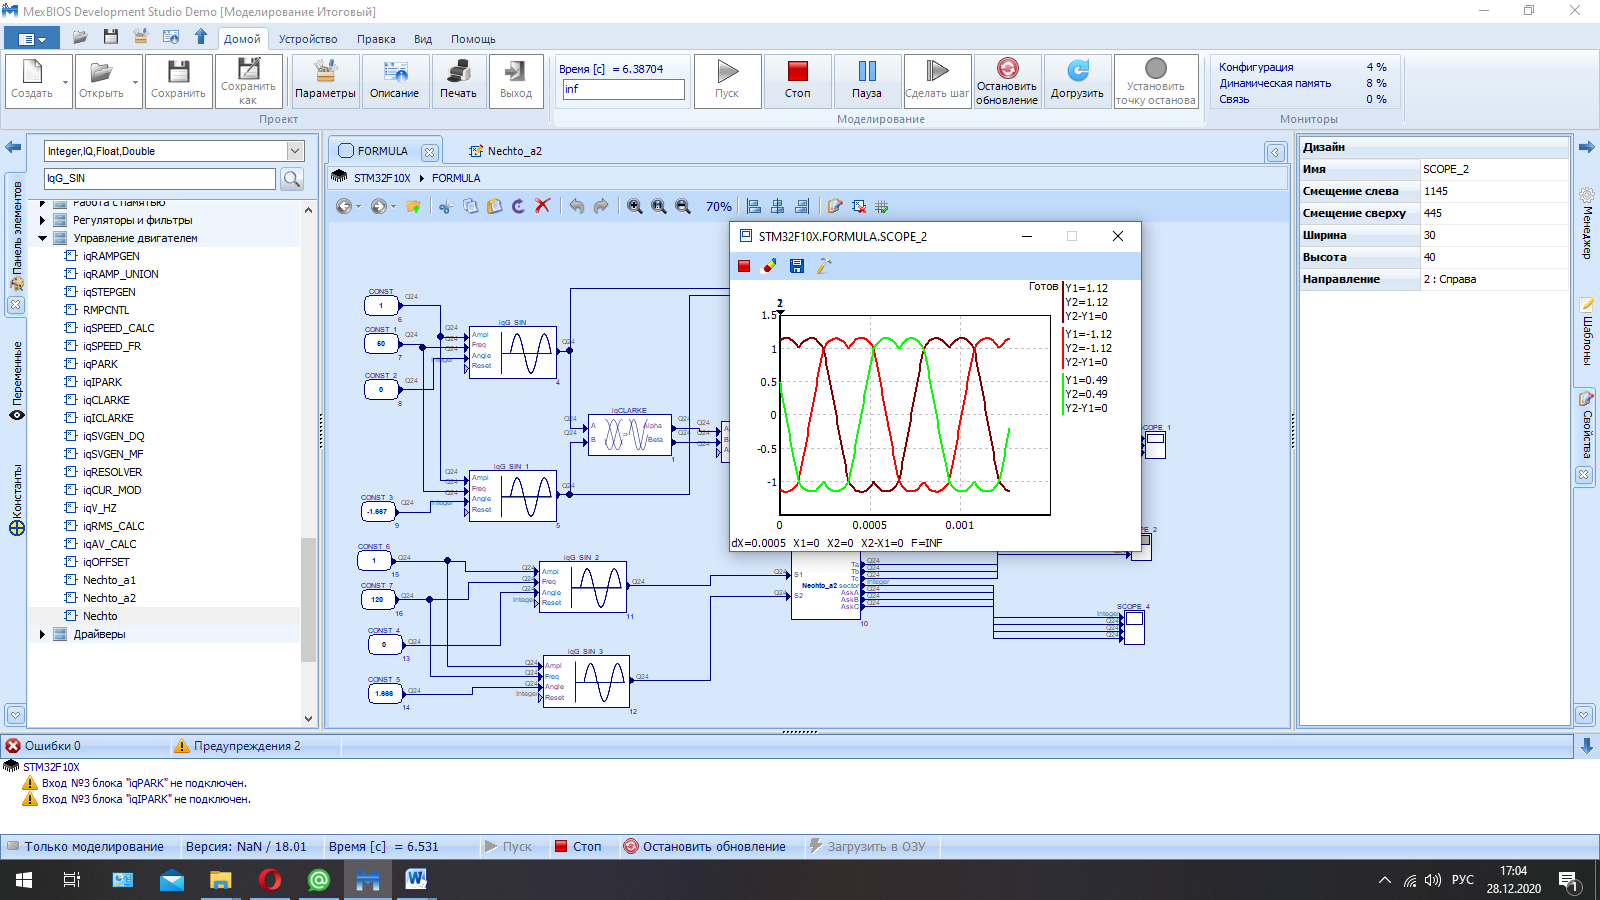
\includegraphics[width=0.75\linewidth]{custom_scope}
\caption{\small проверка алгоритма c использованием ковариантных и контравариантных координат для управления двигателем в среде MexBIOS}
\end{figure}
 \end{frame}

 \begin{frame}
 \frametitle{\begin{tabular}{lp{50pt}r}Фонд оценочных средств&&
\includegraphics[width=0.25\linewidth]{logo2}\end{tabular}}
 \vspace{-0.2cm}
\begin{figure}[ht!]
\centering
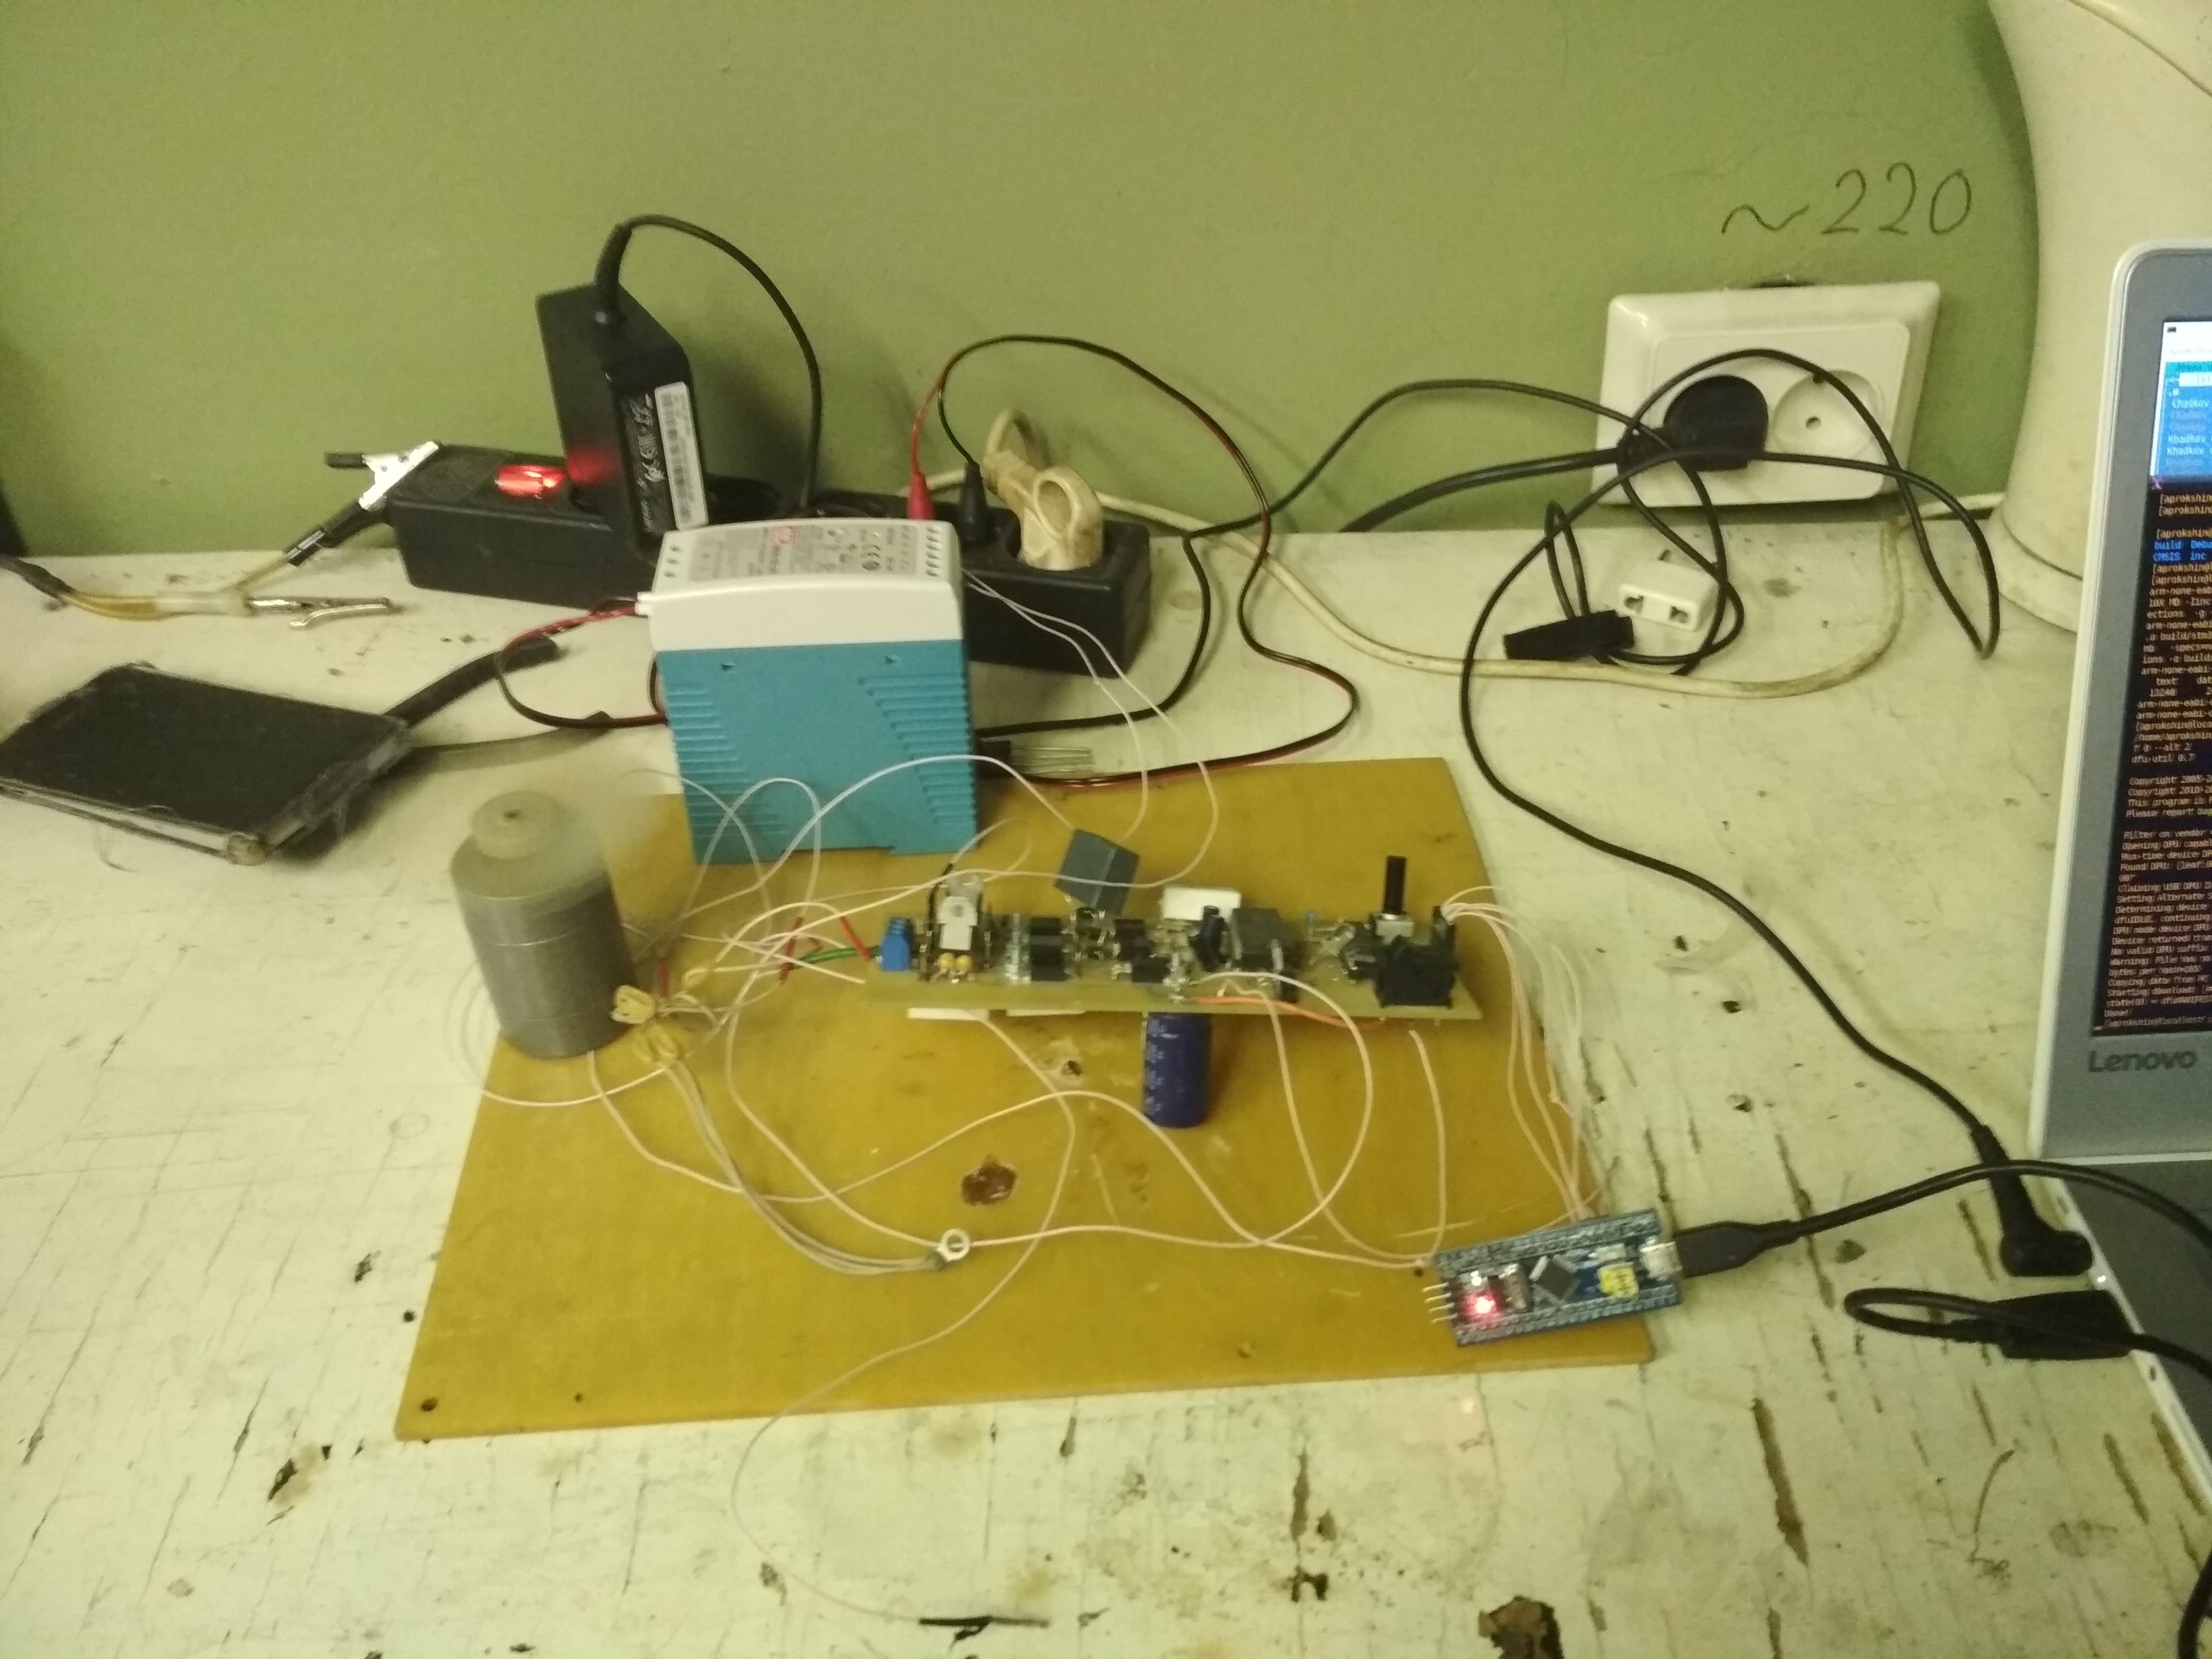
\includegraphics[width=0.58\linewidth]{IMG_20181222_105931}
\caption{результат работы программы на stm32f103c8t6 для кейса №1}
\end{figure}
\end{frame}

 \begin{frame}
 \frametitle{\begin{tabular}{lp{50pt}r}Фонд оценочных средств&&
\includegraphics[width=0.25\linewidth]{logo2}\end{tabular}}
 \vspace{-0.2cm}
\begin{figure}[ht!]
\centering
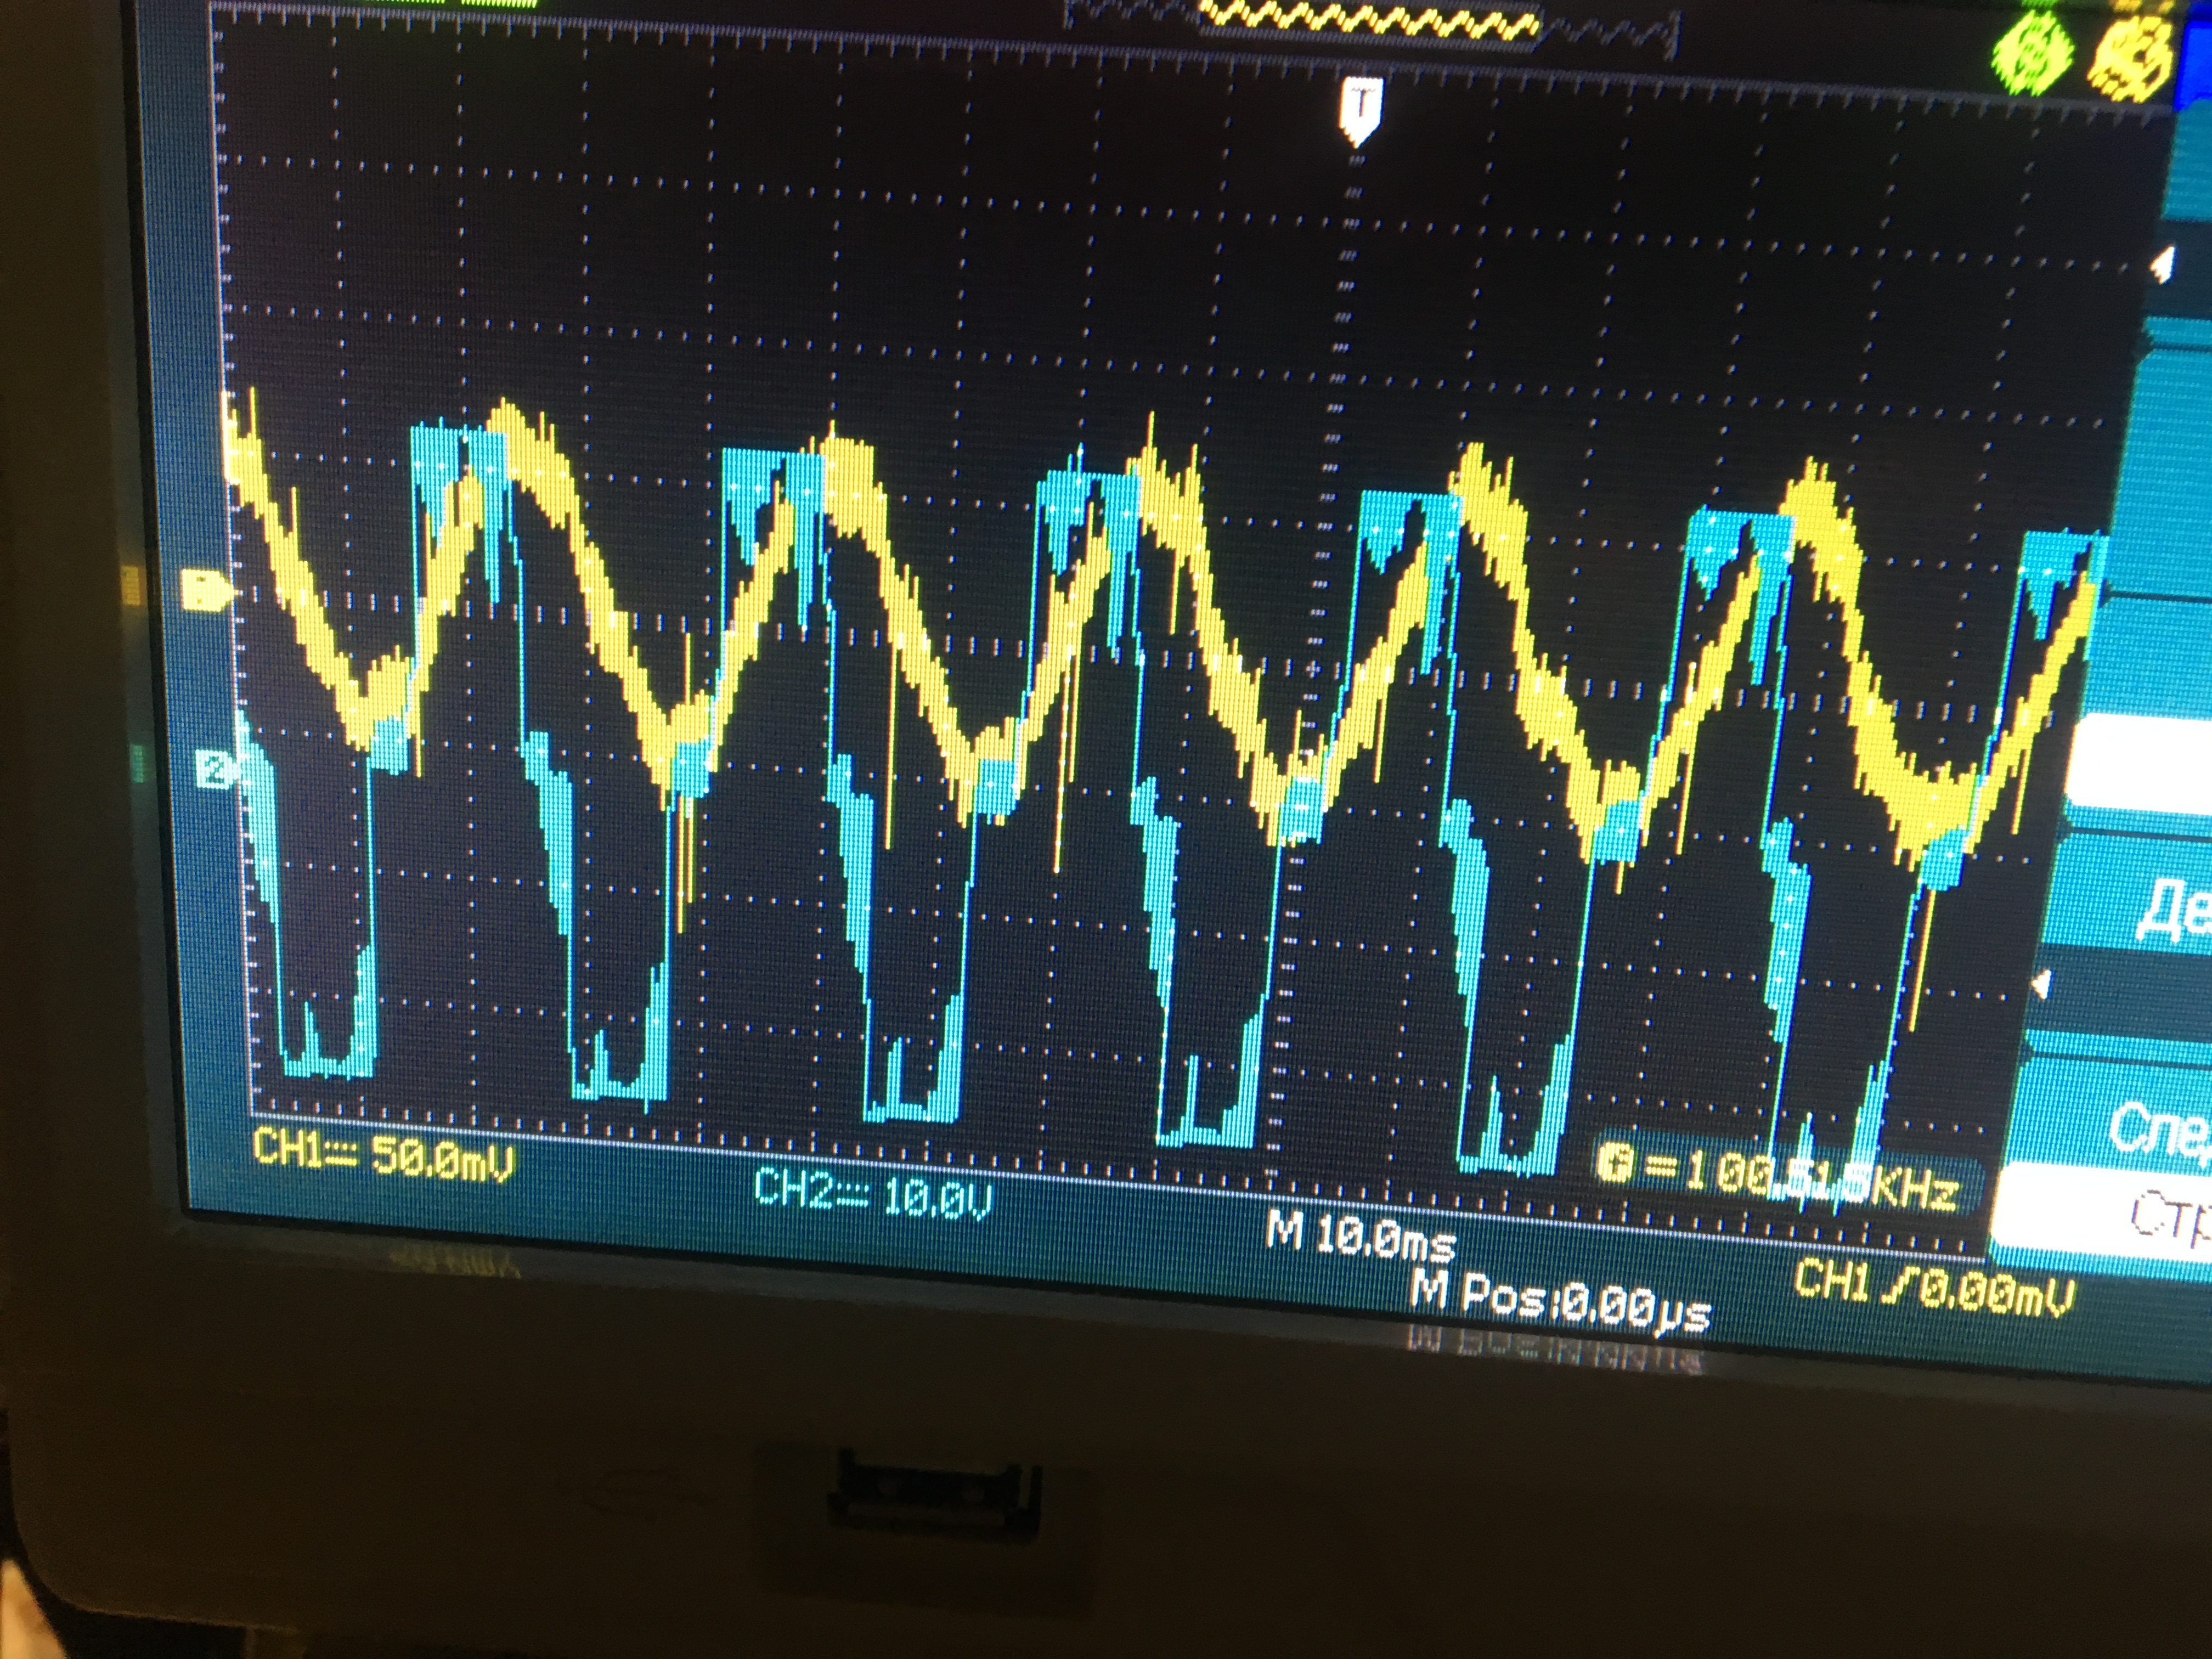
\includegraphics[width=0.58\linewidth]{4IMG_3171}
\caption{\color{yellow}{фазный ток} \color{black}{и} \color{blue}{линейное напряжение} \color{black}{на выходе инвертора}}
\end{figure}
\end{frame}

 \begin{frame}
 \frametitle{\begin{tabular}{lp{0pt}r}\small{Учебно-методическое и информационное обеспечение}&&
\includegraphics[width=0.25\linewidth]{logo2}\end{tabular}}
 \vspace{-1cm}
 \begin{columns}[t]
     \column{1\textwidth}
     \footnotesize

     \begin{exampleblock}{\footnotesize Перечень основной учебной литературы}
\vspace{-0.3cm}
        \begin{itemize}
%           \item \small{\footnotesize{Дубровин Б.А. и др. Современная геометрия, Методы и приложения}}
           \item \small{\footnotesize{
               Прокшин А.Н. и др. 
              \href{https://scm.etu.ru/assets/files/2021/scm21/papers/113-115.pdf} 
              {\colorbox{yellow}{Измерение} тока и напряжения в \colorbox{yellow}{косоугольных координатах} в трехфазной обобщенной электрической машине
               XXIV Международная конференция по мягким вычислениям и измерениям (SCM'2021)}}}
           \item \small{\footnotesize{
               Прокшин А.Н. и др. 
               \href{https://etu.ru/assets/files/university/irvc/konferencii/2019/pps/sbornik-72-pps-2019.pdf}
                { Создание и апробирование \colorbox{yellow}{лабораторных работ по дисциплинам «микроконтроллеры»} и «цифровая и микропроцессорная техника в управлении»
                  Сборник докладов 72 научно-технической конференции ППС, 2019г, с. 134-138}}}
           \item \small{\footnotesize{
               Прокшин А.Н. и др. 
               \href{https://conf-ntores.etu.ru/assets/files/2021/cp/papers/331-332.pdf}
               {\colorbox{yellow}{Создание лабораторных работ} по дисциплине «Цифровая и микропроцессорная техника в управлении» с использованием российского программного обеспечения «MexBIOS Development Studio 6.21»}}}
           \item \small{\footnotesize{
               Прокшин А.Н. и др.
               \href{https://etu.ru/assets/files/university/irvc/konferencii/2018/pps-2018.pdf} 
               {О системах координат для математического описания систем управления электропривода Сборник докладов 71-й научно-технической конференции ППС, СПб, 2018, с.172-175}}}
        \end{itemize}
     \end{exampleblock}
 \end{columns}
 \end{frame}

\begin{frame}
\frametitle{\begin{tabular}{lp{0pt}r}\small{Учебно-методическое и информационное обеспечение}&&
\includegraphics[width=0.25\linewidth]{logo2}\end{tabular}}
 \vspace{-1cm}
 \begin{columns}[t]
     \column{1\textwidth}
     \footnotesize
     \begin{exampleblock}{\footnotesize Перечень основной учебной литературы}
        \begin{itemize}
         \item Соколовский Г.Г. Электроприводы переменного тока с частотным регулированием: Учебник для студ. высш.учеб.заведений.
                -- М. «Академия», 2007 - 272 с.
         \item Ю.Н. Калачев SimInTech: моделирование в электроприводе -- М.изд. ДМК, 2019 -- 95 с.
         \item С.Г.Герман-Галкин и др. Модельное проектирование электромеханических мехатронных модулей движения в среде SimInTech -- M.изд. ДМК, 2020 -- 494 с.
       \end{itemize}
     \end{exampleblock}
 \end{columns}
 \end{frame}


 \begin{frame}
\frametitle{\begin{tabular}{lp{0pt}r}\small{Учебно-методическое и информационное обеспечение}&&
\includegraphics[width=0.25\linewidth]{logo2}\end{tabular}}
 \vspace{-0.5cm}
 \begin{columns}[t]
     \column{1\textwidth}
     \footnotesize
     \begin{exampleblock}{\footnotesize Перечень дополнительной литературы}
        \begin{itemize}
          \item А.А.Горев Переходные процессы синхронной машины -- М.,Л., Гос. энергетическое изд., 1950. -- 551 c.
          \item Программа для векторной широтно-импульсной модуляции для системы управления трехфазной электрической машиной с использованием \colorbox{yellow}{ковариантных и контравариантных координат изображающего вектора}. Свидетельство о государственной регистрации программы для ЭВМ
          \item Программа для системы управления трехфазной электрической машиной c векторной широтно-импульсной модуляцией. Свидетельство о государственной регистрации программы для ЭВМ №2020662398 от 13 октября 2020
          \item \colorbox{yellow}{Веб интерфейс к ngspice} (NG-Spice web interface). Свидетельство о государственной регистрации программы для ЭВМ 
       \end{itemize}
     \end{exampleblock}
 \end{columns}
 \end{frame}



 \begin{frame}
 \frametitle{\begin{tabular}{lp{0pt}r}\small{Учебно-методическое и информационное обеспечение}&&
\includegraphics[width=0.25\linewidth]{logo2}\end{tabular}}
 \vspace{-0.5cm}
 \begin{columns}[t]
    \column{1.0\textwidth}
     \footnotesize
     \begin{exampleblock}{\footnotesize Перечень интернет-ресурсов, необходимых для освоения дисциплины}
       \begin{itemize}
         \item \colorbox{yellow}{\href{overleaf.com}{overleaf} или \href{sharelatex.com}{sharelatex}}
         \item \colorbox{yellow}{\href{github.com}{github}, \href{gitlab.com}{gitlab}, \href{bitbucket.org}{bitbucket}}
         \item \colorbox{yellow}{\href{https://mechatronica-pro.com/ru}{MexBIOS}}
         \item \colorbox{yellow}{\href{https://simintech.ru/}{SimInTech}}
         \item \colorbox{yellow}{\href{https://www.mycompiler.io/new/c}{песочница С}}
         \item \colorbox{yellow}{\href{https://easyeda.com/}{easyEDA}}
      \end{itemize}
     \end{exampleblock}
 \end{columns}
 \end{frame}



% \begin{frame}
% \frametitle{Практические/лабораторные занятия}
% \vspace{-0.5cm}
% \begin{columns}[t]
%     \column{.33\textwidth}
%     \footnotesize
%     \begin{exampleblock}{\footnotesize }
%        \begin{itemize}
%           \item
%        \end{itemize}
%     \end{exampleblock}
%    \column{.33\textwidth}
%     \footnotesize
%     \begin{exampleblock}{\footnotesize }
%       \begin{itemize}
%         \item
%      \end{itemize}
%     \end{exampleblock}
%    \column{.33\textwidth}
%     \footnotesize
%     \begin{exampleblock}{\footnotesize }
%       \begin{itemize}
%         \item
%      \end{itemize}
%     \end{exampleblock}
% \end{columns}
% \end{frame}
% 
% 
% 
% \begin{frame}
% \frametitle{Лекционный блок}
% \vspace{-0.5cm}
% \begin{columns}[t]
%     \column{.50\textwidth}
%     \footnotesize
%     \begin{exampleblock}{\footnotesize }
%        \begin{itemize}
%           \item
%        \end{itemize}
%     \end{exampleblock}
%    \column{.50\textwidth}
%     \footnotesize
%     \begin{exampleblock}{\footnotesize }
%       \begin{itemize}
%         \item
%      \end{itemize}
%     \end{exampleblock}
% \end{columns}
% \end{frame}




\end{document}

